\documentclass[11pt]{report}
\usepackage{hyperref}
\usepackage{apacite}
\usepackage{float}
\usepackage{graphicx}
\usepackage{xcolor}

\usepackage[english]{babel}
\usepackage[utf8x]{inputenc}
\usepackage[a4paper, total={6in, 8in}]{geometry}

% fix the zero section
\renewcommand{\thesection}{\arabic{section}}


\begin{document}


\title{Graph Kernels as Preprocessing for Unsupervised Text Mining Methods}
\author{Levi C. Nicklas}
\date{September 14, 2020}
\maketitle

\section{Abstract}

\hspace*{0.5cm} In this work, a novel text mining method will be explored and developed. Through the use of graph kernels, an emerging topic in data mining and machine learning --- in conjunction with skip-grams and clustering algorithms, a new way to cluster documents is proposed. This method will preserve more information than other standard natural language processing (NLP) and text mining methods, in that it retains the connections and context between words. This method will be applied to various text datasets of varying sources. The performance of graph kernels on graph representations of text data will be compared and assessed. Among the data sources will be social media and technical reports. 

% Rephrasing. Reason: do we know that it will preserve MORE information? If so, how will this be quantified? 




\section{Introduction}

\hspace*{0.5cm} Many modern text mining methods rely on the use of ``bag of words" as their underlying assumptions for their models \cite{nikolentzos2017shortest}. However, these bag of words methods are not consistent with how language functions. The continuous bag of words models fail to preserve the context of words. The methodology proposed in this work will aim to consider the context of words by preserving connections between words. These connections are constructed when two words appear within a fixed window width, $w$. Similar to a bi-gram, where words are considered a pair when they appear adjacent to one another, this is called a ``skip-gram" since words do not need to be adjacent to appear within the window. 

This newly constructed graph of words represents the document from which it came from. When we have many of these graphs, representing a collection of documents, we can compare graphs. One way graphs can be compared is through the use of graph kernels \cite{kriege2020survey}. Graph kernels allow us to construct a measure of similarity between two graphs, and with this new measure we can perform various tasks.

The introduction of the similarity measure allows for classification of graphs, clustering of graphs, and regression. Allowing graph representations of text to be used in typical machine learning methods opens a new way to analyze text data. The particular focus of this work is to study unsupervised methods, specifically tasks related to clustering and outlier detection for text data. The proposed concept is illustrated in Figure \ref{fig:diagram}. \\


\begin{figure}[ht]
\centering

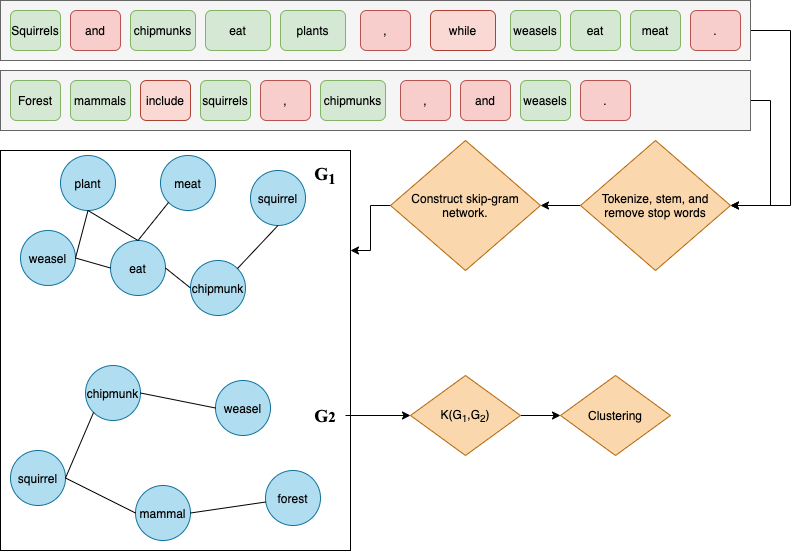
\includegraphics[width = \textwidth]{../../Images/proposal_diagram.png}
\caption{An example of the process described. Two sentences are decomposed into graph structures which are defined by bi-grams. Stop words, in red, are removed.}
\label{fig:diagram}
\end{figure}


\section{Research Questions}

\begin{itemize}

	\item \textit{How do differing styles of text affect graph kernel methods for text mining?}
	\item \textit{Which clustering methods work best with the kernel methods?}
	\item \textit{What modifications can be made to the graph representation to improve clustering results?}

\end{itemize}

\section{Survey of Literature}


The introduction of graph kernels first arose in 2002, from the paper ``\textit{Diffusion kernels on graphs and other discrete structures}" ~\cite{kondor2002diffusion}. Since then, graph kernels have been used in a variety of fields, and modified to suit different problems. These developments have resulted in applications in biology, chemistry, social media analytics, and machine learning. Graph kernels have since formed into 3 large sub-groups: random walk kernels, sub-graph (also called graphlet) kernels, and tree-based methods. Within these three categories there are a multitude of modifications which include things such as edge or vertex attributes into the calculations ~\cite{vishwanathan2010graph}. The graph kernels of particular interest to this study are those which incorporate vertex attributes into the calculation of the kernel.  This inclusion of vertex attributes will allow the assignment of a word from a text document to a vertex. 

The use of graph kernels in text processing has been largely focused on applying them to a neural networks for NLP. However, a 2017 paper by Nikolentzos et.al, covered how their use first arrived at the idea to apply graph kernels to what they called ``graph-of-words" ~\cite{nikolentzos2017shortest}. They utilized a window width to construct a connections between words, effectively ``skipping" some words in between; this concept has also been called a ``skip-gram" network in other contexts ~\cite{cheng2006n}. Members of this research group, and others close to them, have produced software packages to perform some basic graph kernel methods. In addition, there have been a small number of papers from the group about the application of these methods to text mining ~\cite{sugiyama2018graphkernels}. Their work centered around use of neural networks for classification tasks. 



%%% TABLE %%%
\begin{table}[H]
\caption{Summary of Literature Review}
\centering
\begin{tabular}{ c c c c}
\hline
\hline
Topic & Author & Title & Year \\ [0.5ex]
\hline
Graph Kernels & Vishwanathan & Graph Kernels & 2010\\
Graph Kernels & Kriege et al. & A survey on graph kernels & 2020\\
Graph Kernels & Nikolentzos et al. & [graph kernels for doc. similarity] & 2017\\
Graph Kernels & Kondor and Lafferty &  Diffusion Kernels on Graphs [...] & 2002\\
Skip-Grams & Cheng et al. & From n-gram to skipgram [...] & 2006\\
Text Mining & Vazirgiannis et al. & GraphRep: [...] & 2018 \\
Application & Rosenfeld et al. & Kernel of Truth: [...] & 2020\\
Software & Silge and Robinson& tidytext &  2016\\
Software & Sugiyama et al. & graphkernels & 2018 \\
Software & Casardi et al. & igraph & 2013\\


\hline
\end{tabular}

\end{table}

Using a similar framework, the performance of the graph kernels as a pre-processing step for unsupervised learning will be assessed with data sources other than what the originators of the idea used. This assessment will result in validation, or disagreement, with their methods. The data sources will come from social media websites, which will serve as small document size examples, and technical reports from the National Highway and Transportation Safety Administration (NHTSA), which will serve as a larger document size example. The NHTSA data was curated within a research group at Florida Polytechnic University this summer, and the process of data cleaning and transformation is in its final stages for initial exploratory data analysis and tests. This application would appeal to those within the Advanced Mobility Institute (AMI) as a way to text mine these technical documents and identify ``edge cases" within the reports, further supporting the efforts to provide closer to real life scenarios for testing and validation. The social media data will be collected off of reddit, and will remain focused on social health forums on the platform. This will be a continuation of work done at Florida Polytechnic University as well. By text mining these forums, there is an opportunity to better compare comments, threads, or communities at large, thus allowing for additional machine learning processes to take place. 

The work proposed here will center not only on unsupervised methods but also empirical studies on the effectiveness of graph kernels on these types of text data. The effects of varying window width, edge weighting, and document types will be studied. These contributions to the topic will aid in demonstrating the effectiveness on differing document types, and more importantly an exploration into using graph kernels as a preprocessing method for unsupervised learning methods. Using data sources I am familiar with, I will be building upon previous work in unsupervised text mining \cite{akioyamen2020framework}. Data and text mining have been a focus of my education at Florida Polytechnic and this project will be utilizing various skills I have learned through the program. In addition, this work will be relevant to my professional career as well.

%%%%%%%%%%



\section{Deliverables}
\subsection{Description}
The primary deliverable for this study is to contribute to the body of knowledge on graph kernels and their applications. A research article will be prepared showcasing the application of graph kernels in the nontraditional data sources of interest in this work. Through the application examples, others could learn more about applying graph kernels as preprocessing to text data. This paper would be found useful by anyone who does text mining or computational linguistics. The paper produced will be submitted to a relevant journal and/or conference which focuses in computing or the field of application. Other fields which represent additional topics for an application include, but are not be limited to: political science (polarized news or social media), economics (social media reaction to company news), marketing (product reviews/ad reactions), medical (medical dictation notes), psychology (social media and mental health). 

Additionally, an organized and open code repository will be created. This repository would allow the science conducted here to be open to the data science community, and everyone, for their learning and further application. The repository would feature code written to produce examples, and to conduct the research for the publication deliverable (including a copy of the publication for open science). This would not only allow for others to learn the methodology that will be studied here, but also to provide testable code for the community -- promoting a good practice of reproducibility. Providing this code to the community in a transparent and reproducible manner will render this project able to be validated by anyone, and in turn more scientifically sound and welcoming to corrections, additions, and edits. The transparency and openness of this study is of the upmost importance, as it contributes to the growing movement of open science and reproducible research. 



\subsection{Schedule}
 
A tentative schedule with activities for this work is presented in Table \ref{tab:schedule}.


 %%% TABLE %%%
\begin{table}[ht]
\caption{Schedule of Events and Deliverables (Tentative)}
\label{tab:schedule}
\centering
\begin{tabular}{ c c c}
\hline
\hline
Event Number & Activity & Est. Completion Date \\ [0.5ex]
\hline
1 & Literature Review & (Completed) 9/12/20\\
2 & Data Collection and Preparation & (In Prog.)  10/12/21\\
3 & Exploratory Data Analysis & (In Prog.) 10/19/21\\
4 & Preliminary Analysis & 11/2/21\\
5 & Writing and Editing for Publication & 11/23/21\\
6 & Submit to Conference/Journal & 12/31/21\\
7 & Additional Analysis for Thesis & 1/12/21\\
8 & Writing Draft Manuscript & 3/1/21\\
9 & Final Manuscript & 4/1/21\\
10 & Defense & 5/1/21\\
\hline
\end{tabular}

\end{table}
 %%%%%%%%%%




\section{Conclusion}


In summary, a study of the potential of graph kernels as a preprocessing methodology for unsupervised learning techniques will result in a complete master's thesis. Using and developing emerging graph kernel methods, in combination with unsupervised methods that have not been covered extensively, the study will result in contributions to the existing body of knowledge. The proposed framework will be tested using data sources of interest of research groups at Florida Polytechnic University, allowing for sample applications in the fields of data mining and machine learning in health and transportation. Through the production of a publication quality paper, and and a code repository with reproducible results, the conclusions of the research will be available and accessible to groups both inside and outside of the university. With graph kernels being an emerging topic within text mining and NLP, this is important research to undertake; generating additional techniques, applications, and research on graph kernels will help further develop the topic as a whole.  
For the reasons described above, I petition for your approval to pursue this work as my master's thesis.




% ~\cite{vishwanathan2010graph}
%test ~\cite{kriege2020survey}
 %test ~\cite{nikolentzos2017shortest}
%test ~\cite{cheng2006n}
 %test ~\cite{silge2016tidytext}

\nocite{silge2016tidytext}
\nocite{csardi2006igraph}
\nocite{wickham2019welcome}


\bibliographystyle{apacite}
%\bibliographystyle{apalike}
\bibliography{ThesisProposal.bib}
\end{document}